\chapter{Framework}
\label{ch:Framework}

In this chapter the description of the framework development is given. In first sections the conceptual model and the architecture of the solution are discussed. Further sections provide the details of the solution implementation.

\section{Framework Conceptual Model}

The main objective of current thesis work is analyzing ST trajectory data extracted from videos from surveillance cameras and solving the task of identifying outliers. To solve this task the clustering approach was chosen as a basis: firstly trajectory data is used as a training data to define clusters and model them; clusters are denoted as a normal or abnormal ones based on their density; then classifier marks an input trajectory as a normal or anomalous one. 

The contribution of the work is in making an attempt to solve the problem coming from data uncertainty and increase the results accuracy by adapting the algorithm of measuring trajectories similarity:  take into consideration the position of moving objects in respect to the camera. For this purpose a framework covering mentioned tasks was implemented with an ability to extract frequent trajectories and then detect anomalous trajectories.

The basic workflow of the framework consist of processing the input data, calculating the similarity matrix between trajectories, then clustering the trajectories and modeling the extracted clusters, identifying normal and anomalous clusters based on their density, visualization of modeled clusters, and finally taking an input trajectory and classifying it as a normal or abnormal one according to the built clusters' models.

\subsection{Framework Architecture}

The architecture of the framework is based on an already discussed related work \cite{inproceedings:7_related_work} and consists of two phases (\ref{fig:str}):
\begin{itemize}
	\item \textit{offline} to perform clustering and extract frequent trajectories, and
	\item \textit{online} to classify the new trajectory as a normal or abnormal one.
\end{itemize}
\begin{figure}[!htb]
	\centering{}
	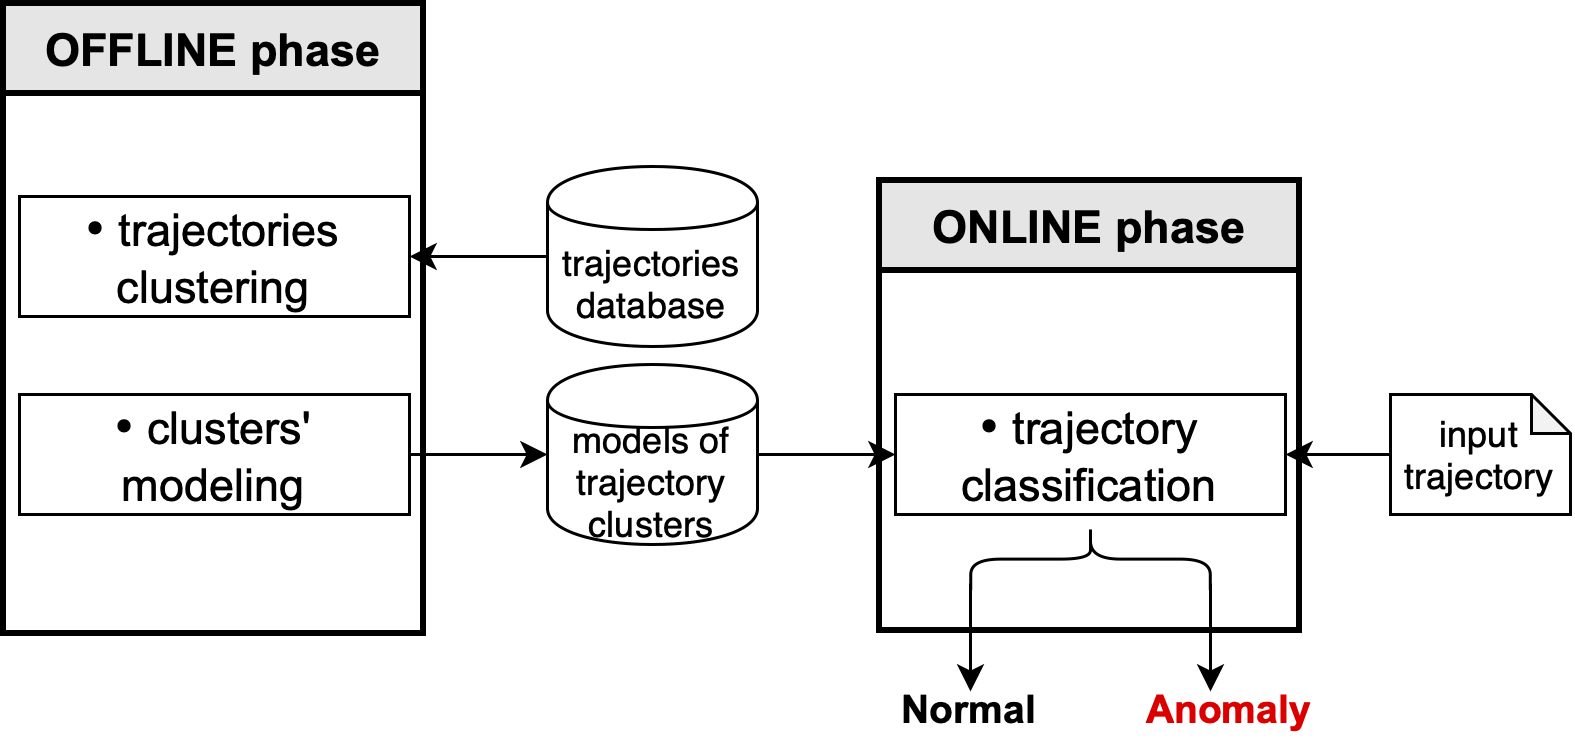
\includegraphics[width=0.8\textwidth]{images/str.png}
	\caption{Two-phased proposed approach}
	\label{fig:str}
\end{figure}

\todo{Add some text about architecture, how should it work}

\subsection{Agglomerative Hierarchical Clustering}

Clustering is done using an unsupervised agglomerative hierarchical clustering approach. The description of this approach is given in Algorithm \ref{algo:ahc-descr} \cite{inproceedings:7_related_work}.

\begin{algorithm}
	\caption{Description of Agglomerative Hierarchical Clustering}
	\label{algo:ahc-descr}
	\SetAlgoLined
	\KwIn{A Database of Trajectories: trajectories}
	\KwOut{Clusters of Trajectories: clusters}
	\textit{Initialization:} \\
	- initialize the clusters with one trajectory in each cluster \\
	\textit{Clusters merging:}\\
	\While{number of clusters is greater than 1}{
		- calculate similarity matrix D between pairs of clusters based on single linkage approach using LCSS similarity measure;\\
		- find the smallest distance between clusters in D;\\
		- merge two clusters with the corresponding smallest distance into a single cluster;\\
		- remove two merged clusters;\\
	}
	
\end{algorithm}

As it was already mentioned, agglomerative hierarchical clustering methods suppose clusters joining, which requires the inter-cluster distance measure to be defined. In \cite{inproceedings:7_related_work} authors have performed evaluation of different linkage methods, including single link, complete link and average link. According to the performed tests, the single link method showed the best results and, in view of this, will be used as a linkage method in the current work.

Single link linkage method considers a minimum distance between two trajectories as an inter-cluster distance and can be summed up as \cite{inproceedings:7_related_work}:

\begin{equation} \label{eq:single_link}
D_{min}(C_i, C_j) = \min_{T_1 \in C_i, T_2 \in C_j} D_{LCSS}(T_1, T_2),
\end{equation} 

where ($C_i$, $C_j$) denote two clusters and ($T_1$, $T_2$) correspond to two trajectories from two clusters respectively.

\subsection{Trajectories similarity}

It was mentioned before, that LCSS distance is used as a distance measure between trajectories to perform clustering. LCSS distance implies computing the Longest Common SubSequence between two input trajectories using two parameter values: $\delta$ and $\varepsilon$. 

Traditionally $\delta$ and $\varepsilon$ parameters are constant and defined in advance. However, in the developed framework in order to handle uncertainty of trajectory data coming from different position in respect to camera adaptive values of parameters are implemented. Parameters are functionally dependent on position of a moving object on a scene in respect to the camera. 

While considering the visualization of trajectories on sample images taken from the cameras, following can be deduced: since the bottom part of the image represent the region located closer to surveillance camera, moving objects on the upper part of the image are more distant from the camera and as a result are more densely located in respect to representation of each other on the image. $\varepsilon$ is responsible for the threshold controlling spatial remoteness of trajectory points while computing similarity distance. Consequently, it must be adapted to the remoteness and decrease as a trajectory point gets farther from the camera.

\todo{$\delta$ behaviour?}

LCSS calculation is described in Algorithm \ref{algo:lcss-descr}.
\todo{include $\delta$ and $\varepsilon$ as an input or calculate inside?}

\begin{algorithm}
	\caption{Description of LCSS distance calculation}
	\label{algo:lcss-descr}
	\SetAlgoLined
	\KwIn{First trajectory: t1,\newline
			Second trajectory: t2,\newline
			Temporal remoteness threshold: $\delta$,\newline
			Spatial remoteness threshold: $\varepsilon$
	}
	\KwOut{LCSS distance for two trajectories}
	\Begin{
		// Initialization \newline
		- calculate length of t1\;
		- calculate length of t2\;
		// LCSS similarity calculation \newline	
		\eIf {t1 or t2 is empty}{
			return 0;	
		}{\eIf {difference between X-coordinates < $\varepsilon$ \newline
			AND difference between Y-coordinates < $\varepsilon$ \newline
			AND difference between trajectory lengths < $\delta$}{
				- increase LCSS by 1\;
				- call recursive for trajectories excluding last points\;
			}{
				- calculate LCSS for first trajectory and second trajectory 	excluding last point\;
				- calculate LCSS for first trajectory excluding last point and second trajectory\;
				- take maximum between these LCSS values\;
			}
		}
		// LCSS distance calculation \newline
		LCSS distance = 1 - LCSS similarity / minimum(input lengths)
	}
\end{algorithm}

\subsection{Measuring the Clusters Validity}

Since the goal of the current work is finding an optimal adaptive parameter values for similarity measure computation, it is necessary to analyze and compare the results after performing clustering. 

According to \cite{online:dunn_cl_valid} cluster validity measures can be classified as follows:
\begin{itemize}
	\item \textbf{Internal cluster validation} -- the result of performed clustering is being evaluated based on the input data clustered. It is based on an internal information and does not include references to external information.
	\item \textbf{External cluster validation} -- evaluation of clustering results is performed in accordance with externally known results, e.g. given class labels. Such validation is not appropriate for unsupervised clustering then no input labels are provided.
	\item \textbf{Relative cluster validation} -- evaluation of the clustering results is done by running the same algorithm using different input parameters, such as number of clusters, etc..
\end{itemize}

At the same time clustering is primarily an unsupervised data mining technique and the input data does not contain data labels. That leads to the necessity to test the resulting clusters in an unsupervised manner. 

One of the most widely used and known measures for evaluating clustering algorithms is a Dunn's Validity Index (DI), which was introduced by J. C. Dunn in 1974 in \cite{article:dunn_orig}. It is an internal evaluation metric which is intended to identify compact clusters with a small variance between cluster members which are well-separated between each other, meaning clusters are sufficiently distant from surrounding clusters in comparison with inter-cluster variance \cite{online:hier_clust_r}. Dunn's index is calculated as the ratio between the minimum inter-cluster distance $d_{min}$ to the maximum intra-cluster diameter $d_{max}$ and for $k$ number of clusters can be defined as follows (Formula \ref{eq:dunn-index}) \cite{article:quant_eval_perf_clust}:

\begin{equation} \label{eq:dunn-index}
	DI = \frac {d_{min}} {d_{max}} = \frac{\min\limits_{\substack{1 \leq i \leq k \\ i+1 \leq j \leq k}} dist(c_i, c_j)} {\max\limits_{1 \leq l \leq k} diam(c_l)}, 
\end{equation}

where minimum inter-cluster distance $d_{min}$ in accordance with the single linkage method refers to the minimal distance between two trajectories from different clusters. Maximum intra-cluster diameter $d_{max}$, or the largest within-cluster distance in other words, supposes computing the diameter of a cluster as the distance between its two farthermost trajectories \cite{inproceedings:clust_ind}. 

Higher values of the DI indicates the better results of clustering. However, the computational cost of the DI шs highly dependent on the data: the computation cost increases with the increase of number of clusters and dimensionality of the data \cite{online:dunn_cl_valid}.

\section{Framework Implementation}

This section will give implementation details of a presented concept based on a chosen stack of technologies. Based on a workflow of the framework outlined above, separate modules will be implemented. Detailed description of each of them will be presented in following sections.

\subsection{Stack of Technologies}

Stack of the technologies description....

.....

.....
\todo{Add stack of technologies}

\subsection{Input Data Description (Nature of Data)}

According to the research done by the US Department of Transportation based on data of Fatality Analysis Reporting System (FARS) and National Automotive Sampling System, nearly 40 percents of all the reported in 2008 year crashes were road intersection related \cite{inproceedings:10_cfi}. Consequently, cross-road transport activity analysis is significantly important nowadays in context of safety, and identifying unsafe vehicular trajectories, which violate traffic rules, may be one of the steps towards improving the statistics.

In the presented work video from enforcement cameras is used for training and testing. Test videos are captured using the Intellectual Transportation Systems implemented on four different Kazan crossroads:
\begin{enumerate}
	\item An intersection of Pravo-Bulachnaya and Puschkina streets (Figure \ref{fig:is_1}).
	\item An intersection of Nesmelova and Kirovskaya Damba streets (Figure \ref{fig:is_2}).
	\item An intersection of Moskovskaya and Galiaskara Kamala streets (Figure \ref{fig:is_3}).
	\item An intersection of Moskovskaya and Parizhskoy Kommunyi streets (Figure \ref{fig:is_4}).
\end{enumerate}

Each crossroad corresponds to a 4-way intersection and is equipped with a single monitoring camera. Sample pictures from surveillance cameras are given below on Figures \ref{fig:is_1} -- \ref{fig:is_4}.
\begin{figure}[!htb]
	\centering{}
	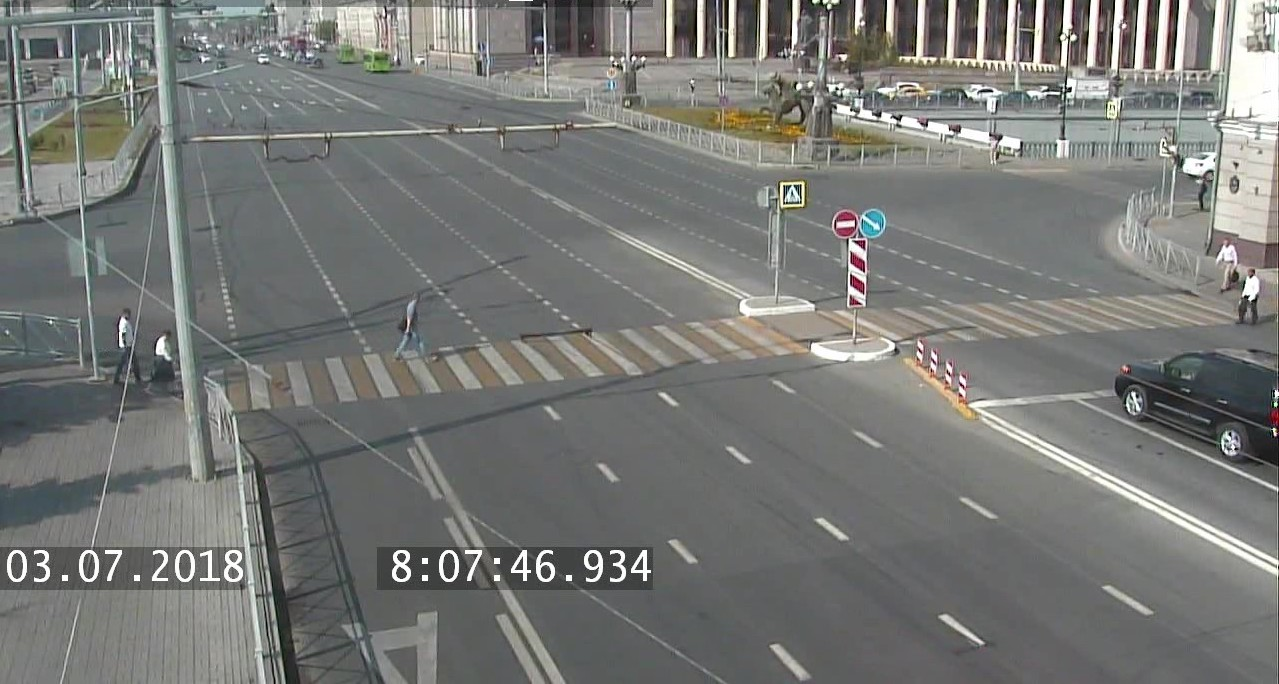
\includegraphics[width=0.8\textwidth]{images/is-1.jpg}
	\caption{Pravo-Bulachnaya / Puschkina intersection}
	\label{fig:is_1}
\end{figure}
\begin{figure}[!htb]
	\centering{}
	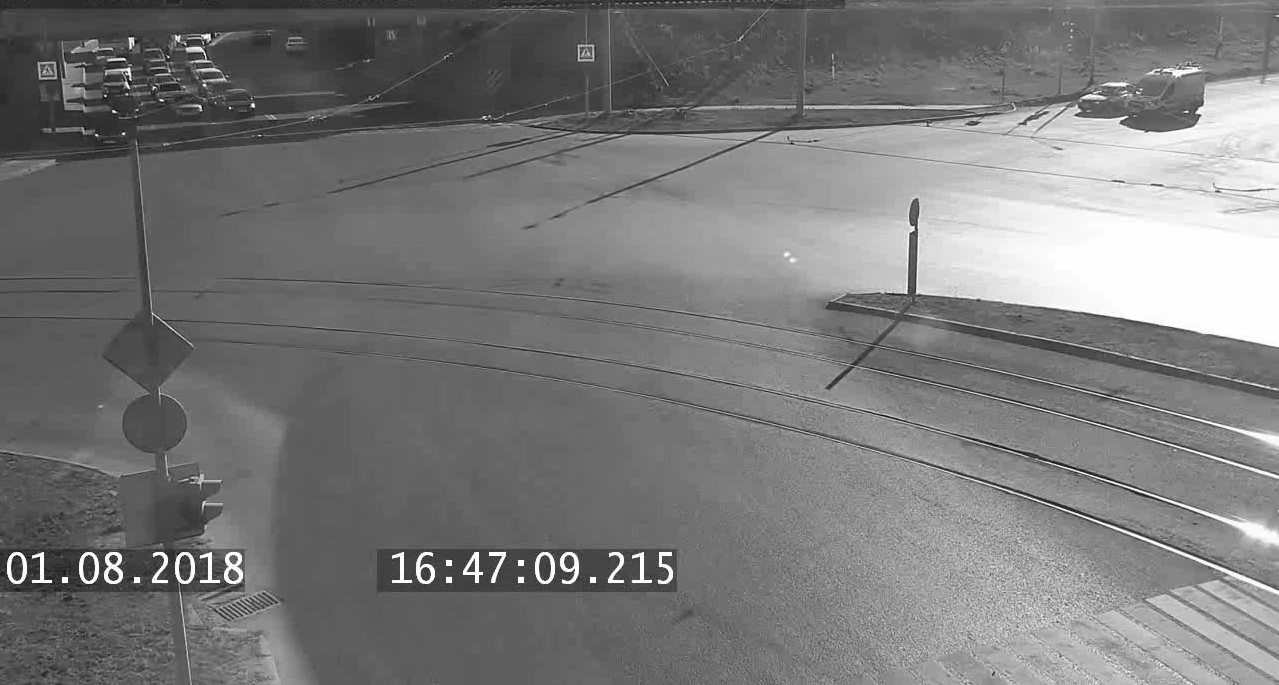
\includegraphics[width=0.8\textwidth]{images/is-2.jpg}
	\caption{Nesmelova / Kirovskaya Damba intersection}
	\label{fig:is_2}
\end{figure}
\begin{figure}[!htb]
	\centering{}
	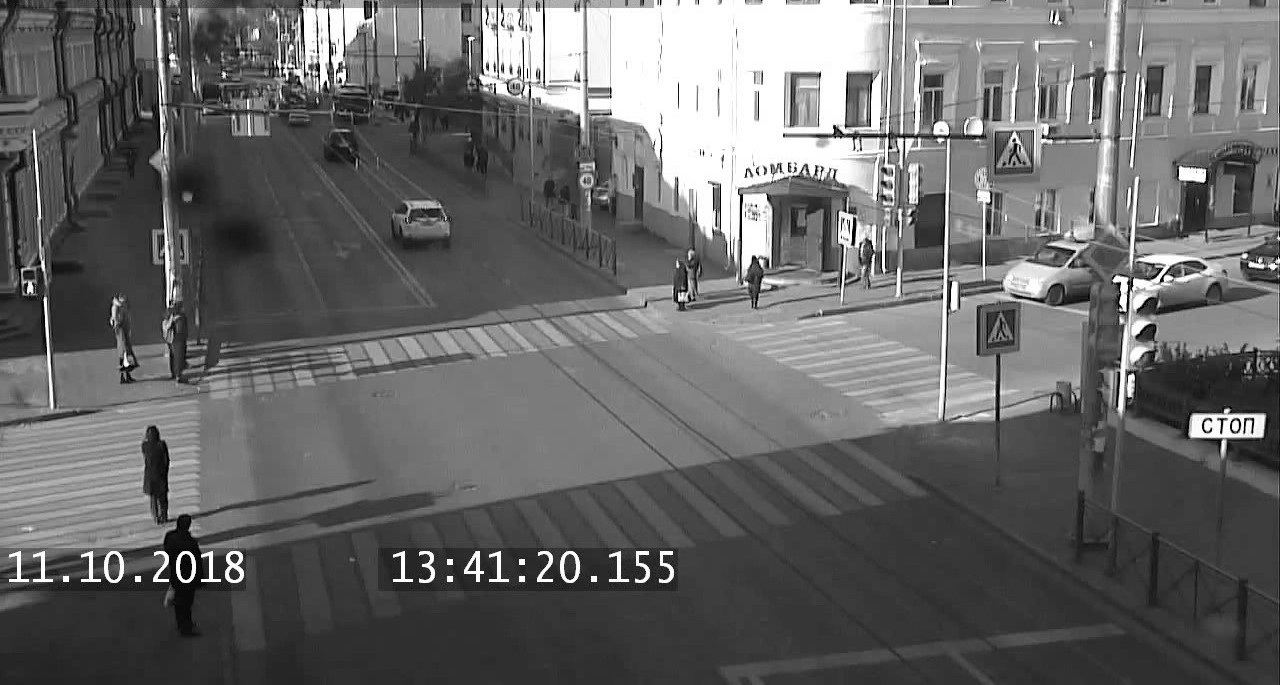
\includegraphics[width=0.8\textwidth]{images/is-3.jpg}	\caption{Moskovskaya / Galiaskara Kamala intersection}
	\label{fig:is_3}
\end{figure}
\begin{figure}[!htb]
	\centering{}
	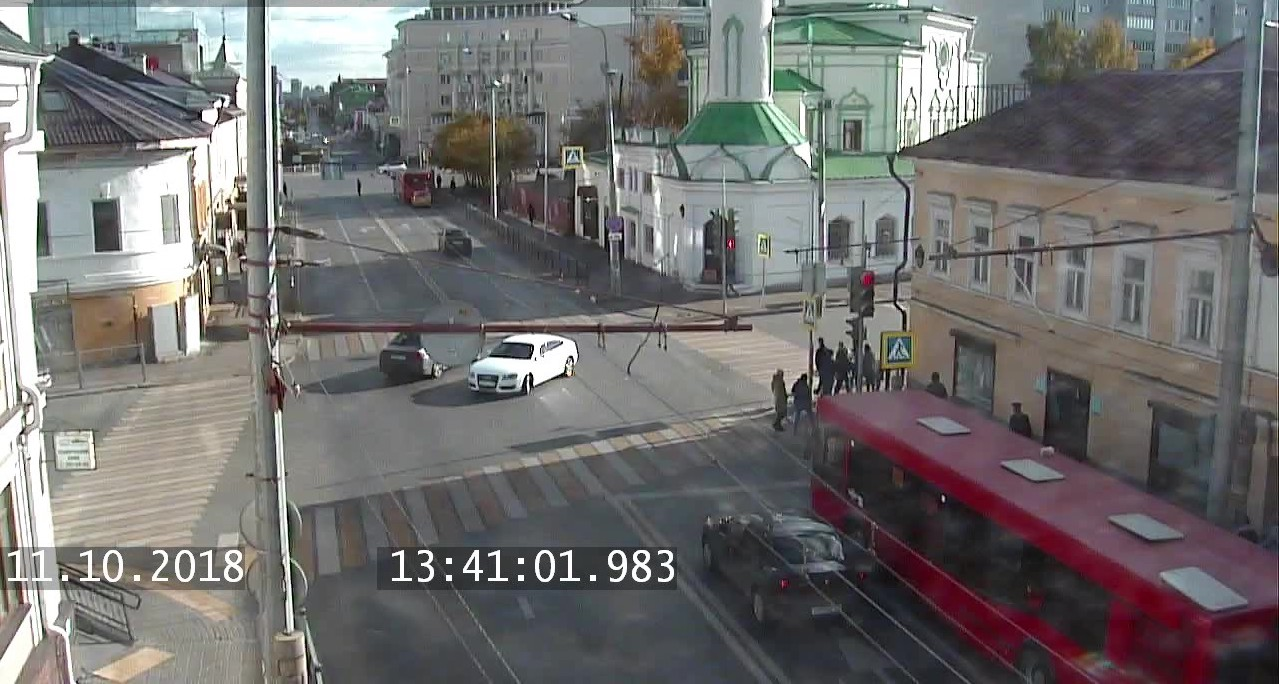
\includegraphics[width=0.8\textwidth]{images/is-4.jpg}
	\caption{Moskovskaya / Parizhskoy Kommunyi intersection}
	\label{fig:is_4}
\end{figure}

Input data files contain 624, 211, 231, 237 vehicular trajectories for the each of the aforementioned intersections respectively.

By a trajectory anomaly we understand vehicle trajectories through the crossroad, which remarkably differ from majority of common, known trajectories. For example, if no turning to the right from the left line is allowed, such a behavior will be unknown and such a trajectory must be considered as an anomaly.

\begin{figure}[!htb]
	\centering{}
	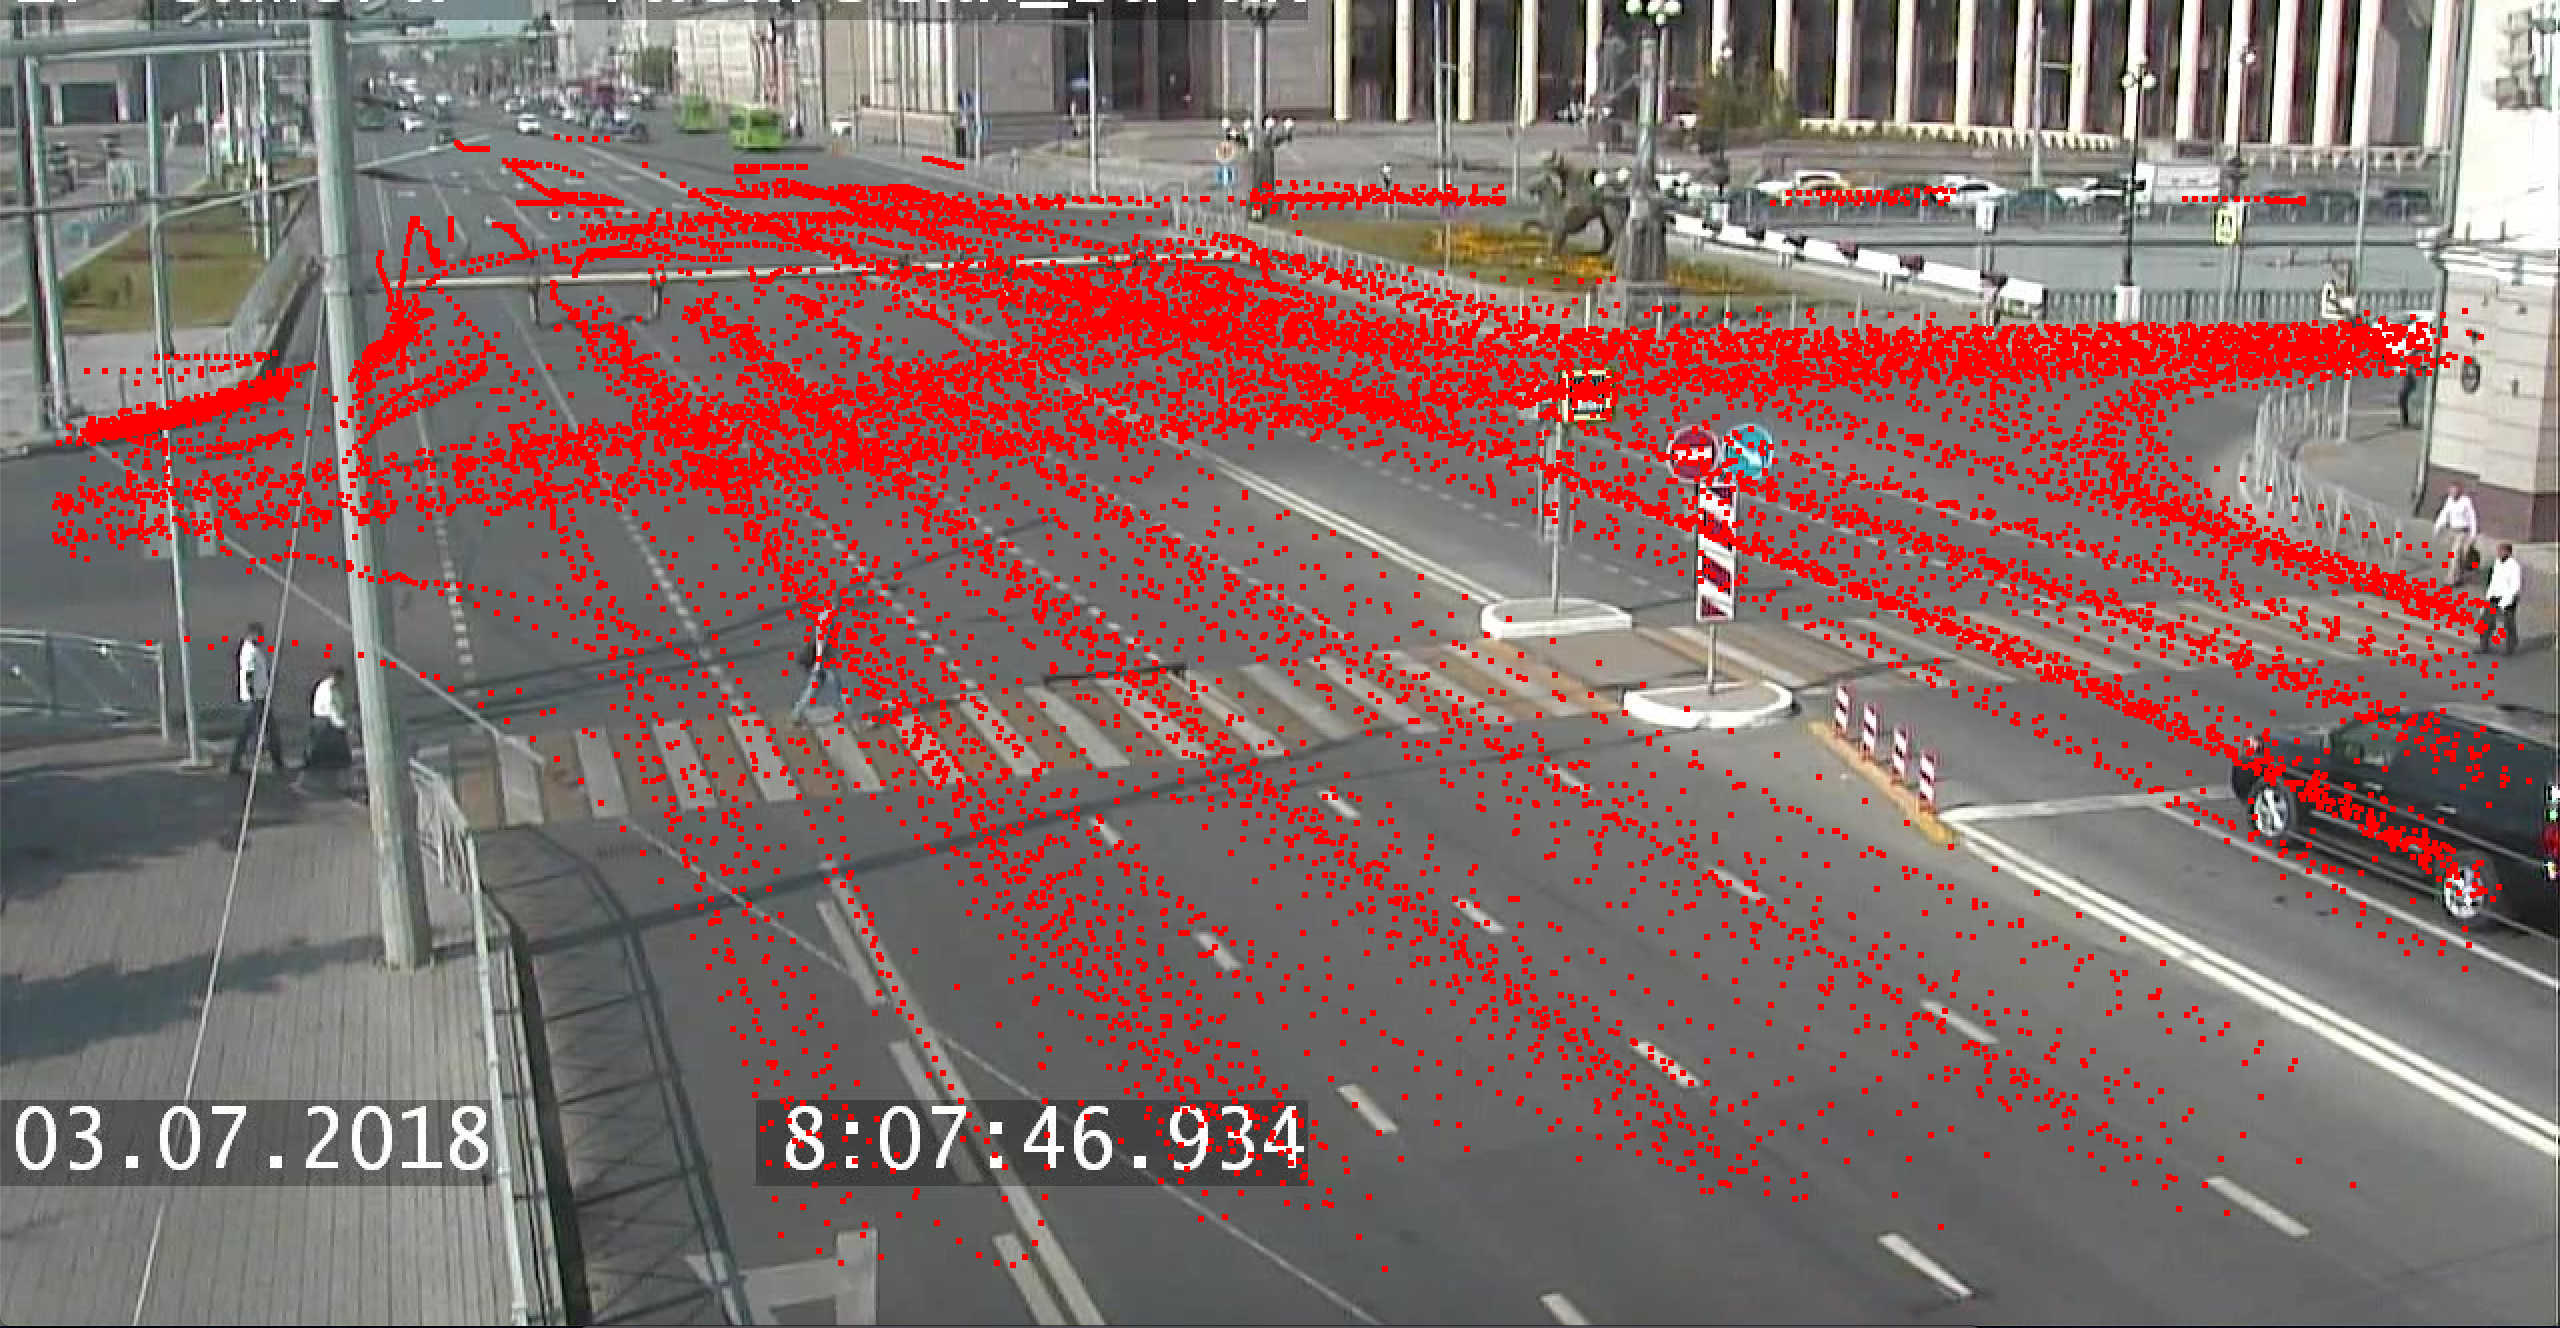
\includegraphics[width=0.8\textwidth]{images/tr-p.png}
	\caption{Output of a tracking system for video the first intersection}
	\label{fig:tr_p}
\end{figure}

\subsubsection{Input data file structure}
Tracking system, as it was described before, handles video from enforcement cameras and prepare it for further analysis: converts video stream into a set of vectors with tracking points on images (Figure \ref{fig:tr_p}).

Input data files have the following structure:
\begin{equation} \label{eq:input_str}
	[[[(x_1^1, y_1^1), ..., (x_1^n, y_1^n)], [t_1, ... t_n]], [[(x_2^1, y_2^1), ..., (x_2^m, y_2^m)], [t_1, ... t_m]], ...]
\end{equation}

As it can be seen from the input data file structure, each trajectory is represented by a two-element array, where first array stores coordinates as an array of two-tuples $(x_i^j, y_i^j)$ and second array contains timestamps for each spatial point in the corresponding order $(t_i)$. The extracted $x$- and $y$-coordinates correspond to pixels on input images. In Formula \ref{eq:input_str} the lower index of the spatial coordinates indicates the ordering number of a trajectory, while the upper index indicates the ordering number of a tracking point. The outer array refers to the array of trajectories.

\subsection{Input Data Processing}
Since chosen algorithm requires trajectories in a form of multi-dimensional vectors, the initial input data needs to be converted into the required form. For that reason, a custom parser was implemented. It takes a ‘txt’ file with trajectories as an input and as a result it returns a list of Trajectory objects. Trajectory object consists of a number of TrajectoryPoint objects with following information: \textit{x}-coordinate, \textit{y}-coordinate, time \textit{t}. The source code of the parsing method is presented in the Listing in Appendix chapter.

As it was mentioned before, the current work is focused on detecting two types of abnormalities: spatial and spatiotemporal. To detect the outliers of the first group it is sufficient to analyze spatial information of trajectories. Detecting outliers of the second group, which is formed by trajectories of vehicles moving with an anomalously low or high speed, requires taking into consideration the temporal information along with spatial. For that reason the average constant speed $\upsilon$ is being calculated for each of the input trajectories $t$ at the end of the parsing step using the following equation (Formula \ref{eq:avg_speed}):

\begin{equation} \label{eq:avg_speed}
\upsilon_{avg}(t) = \frac{distance_{total}} {time_{total}},
\end{equation}

where $distance_{total}$ refers to the total distance between the first and last trajectory points and $time_{total}$ refers to the time elapsed. The total distance can be computed as a sum of Euclidean distances between trajectory points on neighboring frames. Since it is known that frames are taken with an inter-frame interval 0,01 second, the speed calculation can be implemented as follows (Listing \ref{lst:speed-calc}):

\lstset{style=code-style-java}
\lstinputlisting[caption={Speed calculation}, label={lst:speed-calc}] {listings/calcSpeed.java}


\subsection{Similarity measure calculation}

As it was mentioned before, LCSS measure will be used as a similarity measure. Consequently, LCSS distance will be calculated based on a LCSS similarity according to above mentioned formulas. It is worth noting that LCSS distance is symmetric and for pair of trajectories can be computed just once \cite{inproceedings:28_lcss_dsmt}.

Notwithstanding that the implementation of LCSS similarity measure exists in R package \cite{online:r_lcss}, it does not allow $\delta$ and $\varepsilon$ parameters to be dynamic. For that reason the custom implementation was written. The method for LCSS calculation is presented in \ref{lst:lcss-calc}. 

\lstset{style=code-style-java}
\lstinputlisting[caption={LCSS calculation}, label={lst:lcss-calc}] {listings/calcLCSS.java}

\subsection{Clustering}



\subsection{Clusters' modeling}